\documentclass{beamer}
\usepackage{ctex, hyperref}
\usepackage[T1]{fontenc}

% other packages
\usepackage{latexsym,amsmath,xcolor,multicol,booktabs,calligra}
\usepackage{graphicx,pstricks,listings,stackengine}

\author{杨景媛}
\title{婚姻匹配与生育对妇女遭受家庭暴力的影响}
\subtitle{毕业设计开题报告}
\institute{武汉大学经济与管理学院}
\date{2023年8月20日}
\usepackage{whu}

% defs
\def\cmd#1{\texttt{\color{red}\footnotesize $\backslash$#1}}
\def\env#1{\texttt{\color{blue}\footnotesize #1}}
\definecolor{deepblue}{rgb}{0,0,0.5}
\definecolor{deepred}{rgb}{0.6,0,0}
\definecolor{deepgreen}{rgb}{0,0.5,0}
\definecolor{halfgray}{gray}{0.55}

\lstset{
    basicstyle=\ttfamily\small,
    keywordstyle=\bfseries\color{deepblue},
    emphstyle=\ttfamily\color{deepred},    % Custom highlighting style
    stringstyle=\color{deepgreen},
    numbers=left,
    numberstyle=\small\color{halfgray},
    rulesepcolor=\color{red!20!green!20!blue!20},
    frame=shadowbox,
}


\begin{document}

\kaishu
\begin{frame}
    \titlepage
    \begin{figure}[htpb]
        \begin{center}
            
\includegraphics[width=0.2\linewidth]{pic/whulogo.png}
        \end{center}
    \end{figure}
\end{frame}

\begin{frame}
    \tableofcontents[sectionstyle=show,subsectionstyle=show/shaded/hide,subsubsectionstyle=show/shaded/hide]
\end{frame}

\section{选题背景}
\begin{frame}{家暴概况}
    \begin{itemize}[<+-| alert@+>] 
        \item 针对妇女的暴力行为是世界范围内的普遍现象:全球近35\%的妇女自15岁起就遭受过亲密伴侣或非伴侣的暴力行为(WHO,2013)。
        \item 在中国,根据中国社会科学院的数据,近30\%的家庭成员遭受过不同程度的家庭暴力,其中90\%的施暴者为男性。
        \begin{figure}
            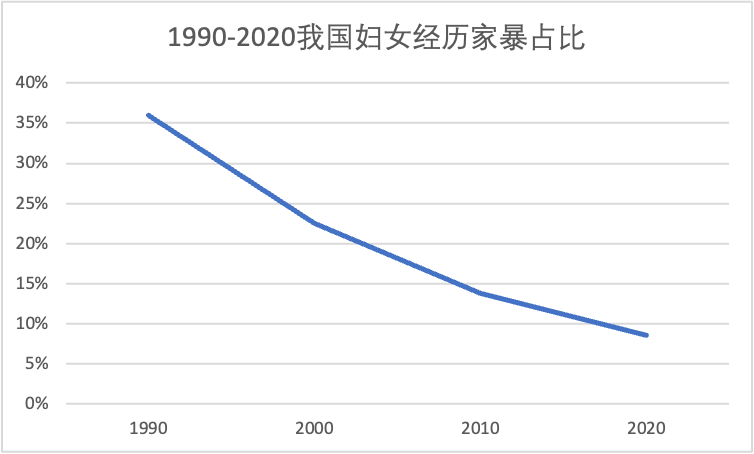
\includegraphics[scale=0.5]{历年家暴占比.png}
        \end{figure}
    \end{itemize}
\end{frame}

\begin{frame}{家暴治理现状}
    \begin{itemize}[<+-| alert@+>] 
        \item 国外:《单边离婚法案》
        \item 国外:《立即逮捕法案》
        \item 我国:2015年通过《反家庭暴力法》
        \item 但根据陈洪磊与陈明静(2022)对3961份家暴裁判文书的分析,当前对家暴行为的司法救济仍然存在对准家庭暴力主体范围和家庭暴力行为的界定分歧、对人身安全保护令法定签发条件的适用困惑、司法惯性与释法说理欠缺以及受害方举证困难等适用问题。
    \end{itemize}
\end{frame}

\section{文献综述}
\begin{frame}{家庭暴力}
    \begin{itemize}[<+-| alert@+>] 
        \item 从家庭内部处出发,讨论在家庭内部导致家暴的成因。
        \begin{itemize}
            \item 家庭议价权的上升可能降低了被家暴的风险;\\ 受教育水平、就业状况等都有可能影响到婚内议价权
            \item 但家庭议价权的上升也可能提高被家暴的风险;\\ 基于“a lost authority or gender identity as the “family provider”的报复行为
            \item 家暴并不是议价权博弈的结果,而是分配资源的手段
        \end{itemize}
        \item 从家庭外部出发,讨论怎样的政策可以有效减少家暴
        \begin{itemize}
            \item 效果待定的政策——干预暴力行为本身
            \item 实证有效的政策——提高议价权
        \end{itemize}
    \end{itemize}
\end{frame}


\begin{frame}{女性生育与就业}
    一般认为,生育与女性的劳动参与是相互影响的,女性在生育和养育孩子方面所花费的时间和精力会限制其就业行为;而女性劳动参与率的提高也会促使生育率下降;
    \begin{itemize}[<+-| alert@+>] 
        \item 心理和社会因素对劳动力市场性别差距的影响;
        \item 男性收入、社会习俗对待女性工作的态度、家庭结构和家庭照料均是影响女性劳动供给的重要原因;
        \item 新中国成立以来,我国女性的劳动参与率一直领先世界前列,但自20世纪90年代以来出现下降;
        \item 然而在排除受教育水平提高等其他因素后,女性生育率下降的趋势依然存在。
    \end{itemize}
\end{frame}

\begin{frame}{婚姻匹配}
    \begin{itemize}[<+-| alert@+>] 
        \item Becker(1973,1974)用经济学理论来解释了婚姻市场的匹配,他给出了一个静态的、效用可以转移的模型来解释,只有当男女的某些特征(如家庭、收入等)在家庭生产中属于互补品时,则具有相似特征的男女会匹配在一起,如果这些特征是属于替代品,那么这些特征差异较大的男女会匹配在一起;
        \item 由于在养育孩子投入中自然的在性别差异,使得男女在婚姻匹配上存在不同偏好;
        \item 丈夫和妻子的相对收入高低会影响妻子的劳动参与率、收入水平以及双方的婚姻满意度;————社会观念预设的身份(性别)角色。
    \end{itemize}
\end{frame}

\section{研究意义}
\begin{frame}
    \begin{itemize}[<+-| alert@+>] 
        \item 补充了我国在家庭暴力领域的研究空白,尤其分析了由生育政策带来的冲击对妇女经历家暴的影响;
        \item 系统分析我国女性家庭议价权与经历家暴概率的关系(目前关于国内的两篇文献都认为婚内议价权的提高会降低家暴概率)
        \item 分析社会观念在其中的作用(生育观念、婚姻匹配倾向)
        \item 讨论对女性的人力资本投入是否能有效改善女性福利
    \end{itemize}
\end{frame}

\section{数据与实证策略}
\begin{frame}{数据介绍}
    本文使用的数据来自全国妇联和国家统计局分别与1990年、2000年以及2010年开展的中国妇女社会地位调查。调查问卷旨在全面反映中国妇女的社会经济状况,包括健康、教育、经济、生活方式、合法权益、价值观以及态度等。\\
    选择受访者为已婚女性的样本。(平均每年约1-2万)
    \begin{itemize}[<+-| alert@+>] 
        \item 对于被解释变量的定义:是否经历家暴
        \begin{itemize}
            \item 主回归:配偶是否有过殴打行为?
            \item 稳健型检验:将家暴行为扩大到:情感虐待、是否强迫性生活等
        \end{itemize}
        \item 对于被解释变量的定义:
        \begin{itemize}
            \item 生育:定义1.是否生育;2.生育子女数量
            \item 婚姻匹配:定义婚姻匹配度
        \end{itemize}
    \end{itemize}
\end{frame}

\begin{frame}{不同组别生育孩子数量}
    \begin{figure}
        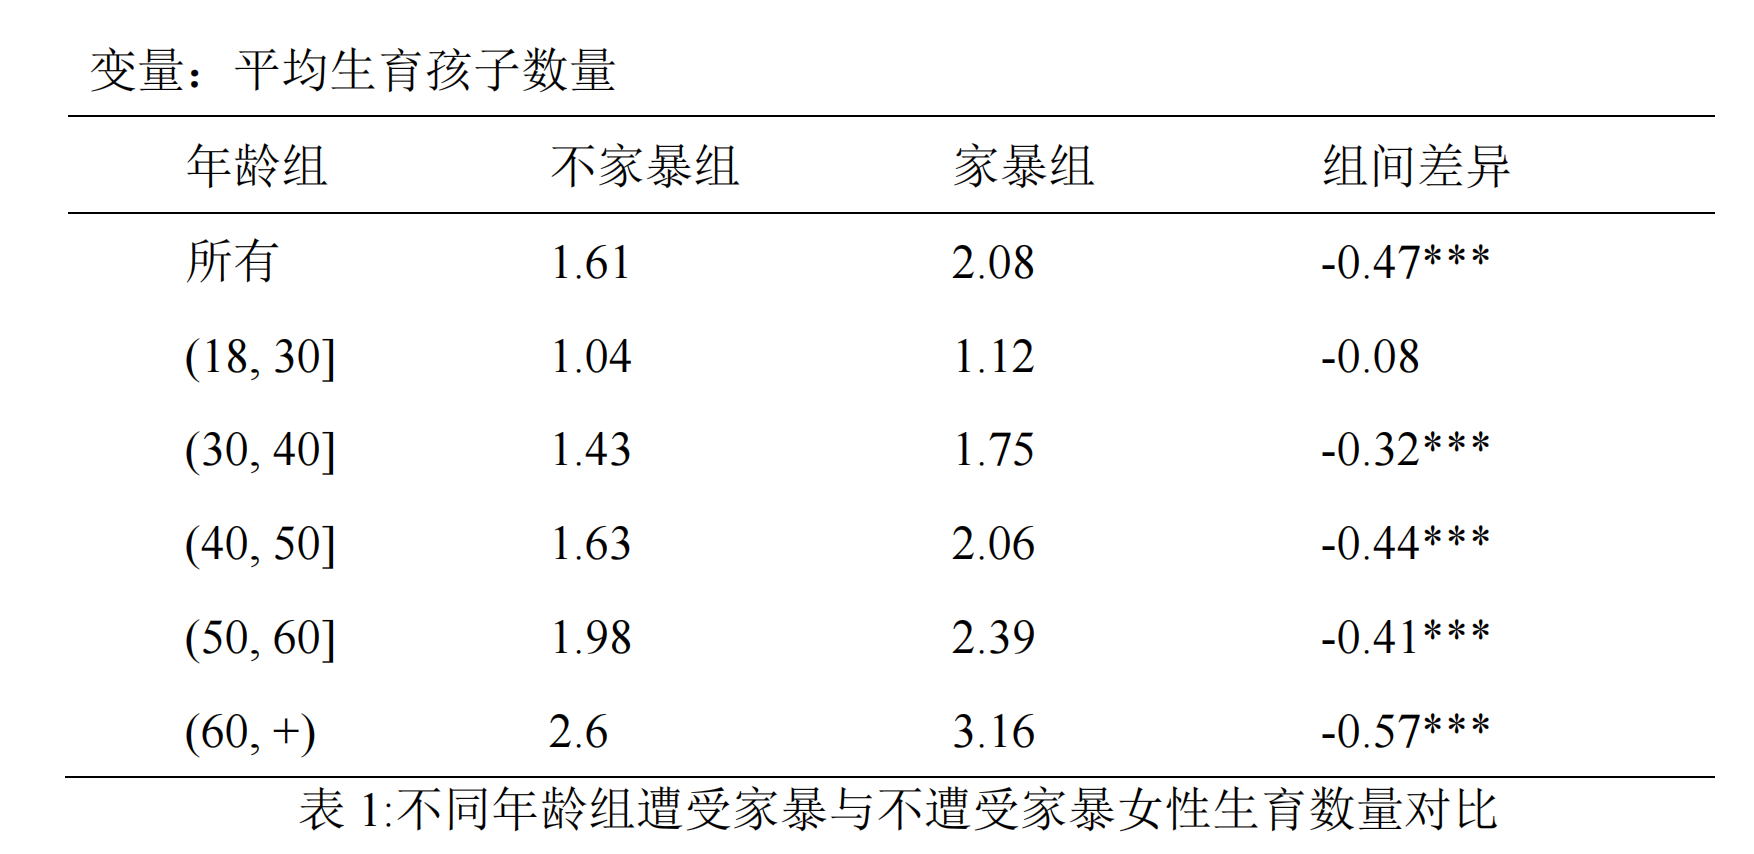
\includegraphics[scale=0.35]{1.png}
    \end{figure}
\end{frame}

\begin{frame}{婚姻匹配与妇女遭受家庭暴力}
    \begin{figure}
        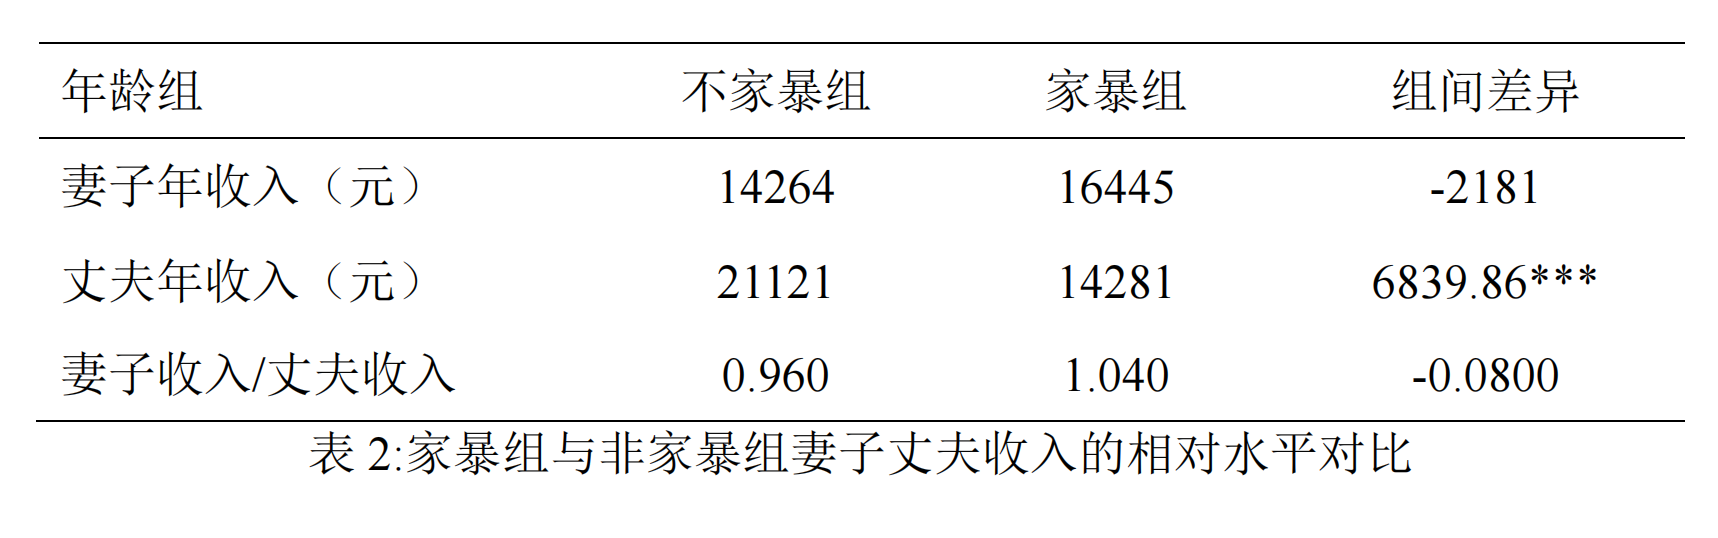
\includegraphics[scale=0.35]{2.png}
    \end{figure}
\end{frame}

\begin{frame}{婚姻匹配与妇女遭受家庭暴力}
    \begin{figure}
        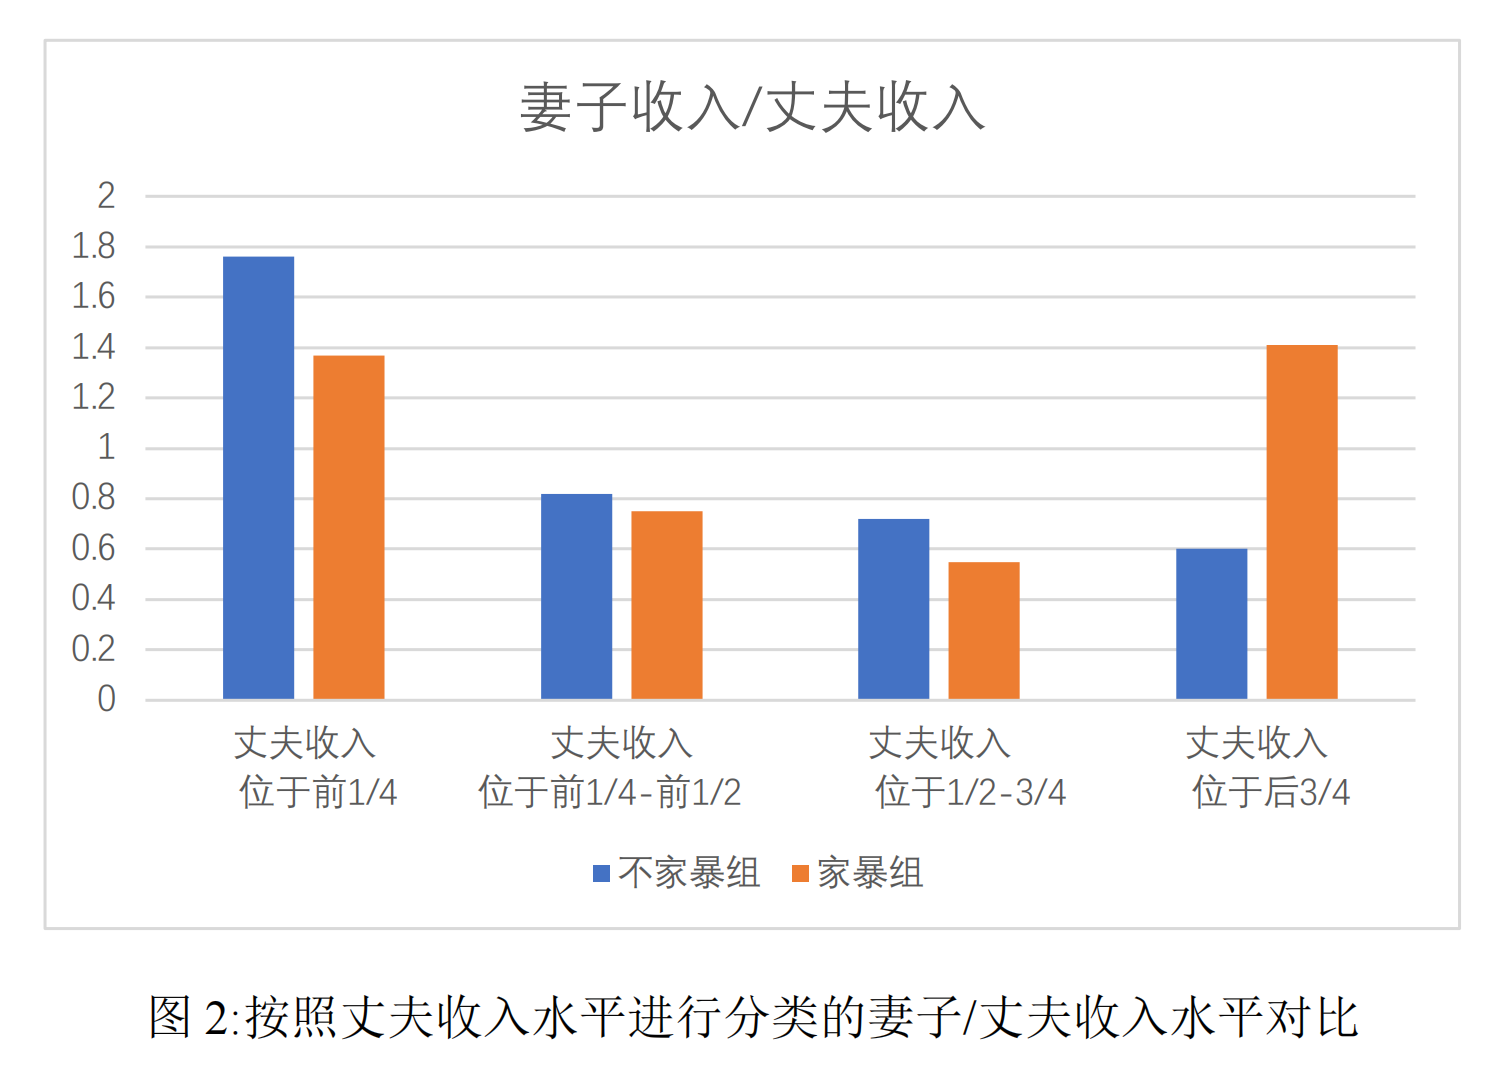
\includegraphics[scale=0.35]{3.png}
    \end{figure}
\end{frame}

\begin{frame}{实证策略-生育}
    \begin{itemize}[<+-| alert@+>] 
        \item OLS估计方程:\\
        \begin{equation}
            Abuse_{ijt}=β_0+β_1 Fertility_{ijt}+X_{ijt}+γ_j+μ_t+ε_{ijt}
        \end{equation}
        \item IV选取:
        \begin{itemize}
            \item 计划生育政策罚款
            \item 头胎子女性别
        \end{itemize}
    \end{itemize}
\end{frame}

\begin{frame}{实证策略-婚姻匹配}
    \begin{itemize}
        \item OLS估计方程:\\
        \begin{equation}
            Abuse_{ijt}=\beta_0+\beta_1 Match_{ijt}+X_{ijt}+γ_j+μ_t+ε_{ijt}
        \end{equation}
    \end{itemize}
\end{frame}

\begin{frame}
    \begin{center}
        {\Huge\calligra Thanks!}
    \end{center}
\end{frame}

\end{document}